\documentclass[tikz,border=8pt]{standalone}
% Shared look for every TikZ diagram. Load with \input{../../tools/tikz-style.tex}
\usepackage[T1]{fontenc}
\usepackage{lmodern}
\renewcommand{\sfdefault}{lmr}  % diagrams use the same serif as the text
\usetikzlibrary{arrows.meta, positioning, shapes.geometric, calc, fit, backgrounds}
\definecolor{cblue}{HTML}{4C78A8}
\definecolor{corange}{HTML}{F58518}
\definecolor{cgreen}{HTML}{54A24B}
\definecolor{cred}{HTML}{E45756}
\definecolor{cpurple}{HTML}{B279A2}
\definecolor{cgrey}{HTML}{6B6B6B}
\tikzset{
  every picture/.style={font=\sffamily, line width=1.2pt},
  box/.style={draw=#1, fill=#1!12, rounded corners=4pt, align=center, inner sep=7pt, minimum height=1.1cm},
  box/.default=cgrey,
  arrow/.style={-{Stealth[length=3mm]}, draw=cgrey, line width=1.4pt},
  title/.style={font=\sffamily\bfseries\Large},
  note/.style={font=\sffamily\small, text=cgrey, align=center},
}
\AtBeginDocument{\hyphenpenalty=10000 \exhyphenpenalty=10000}

\begin{document}
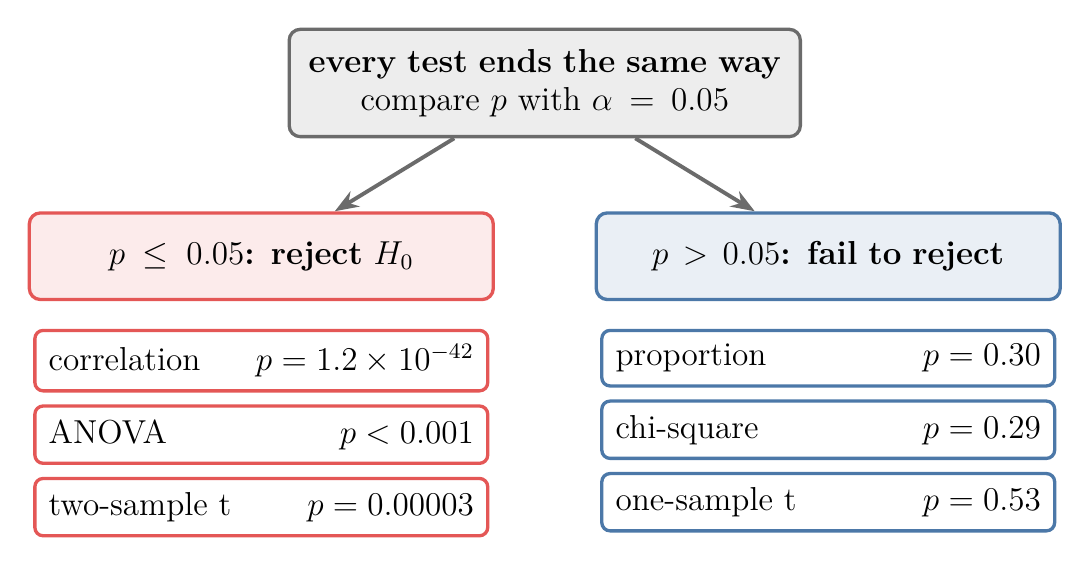
\begin{tikzpicture}[every node/.append style={font=\sffamily\large}, t/.style={draw=#1, fill=white, rounded corners=3pt, text width=5.4cm, inner sep=5pt, line width=1.2pt}]
  \node[box=cgrey, text width=6cm] (all) at (3.6,0) {\textbf{every test ends the same way}\\ compare $p$ with $\alpha = 0.05$};
  \node[box=cred, text width=5.4cm] (rej) at (0,-2.2) {\textbf{$p \le 0.05$: reject $H_0$}};
  \node[box=cblue, text width=5.4cm] (keep) at (7.2,-2.2) {\textbf{$p > 0.05$: fail to reject}};
  \draw[arrow] (all) -- (rej); \draw[arrow] (all) -- (keep);
  \node[t=cred, below=0.35cm of rej] (r1) {correlation \hfill $p = 1.2 \times 10^{-42}$};
  \node[t=cred, below=0.15cm of r1] (r2) {ANOVA \hfill $p < 0.001$};
  \node[t=cred, below=0.15cm of r2] (r3) {two-sample t \hfill $p = 0.00003$};
  \node[t=cblue, below=0.35cm of keep] (k1) {proportion \hfill $p = 0.30$};
  \node[t=cblue, below=0.15cm of k1] (k2) {chi-square \hfill $p = 0.29$};
  \node[t=cblue, below=0.15cm of k2] (k3) {one-sample t \hfill $p = 0.53$};
\end{tikzpicture}
\end{document}
